%!TEX TS-program = sage

\documentclass[11pt]{amsart}
\usepackage{geometry}                % See geometry.pdf to learn the layout options. There are lots.
\geometry{letterpaper}                   % ... or a4paper or a5paper or ... 
%\geometry{landscape}                % Activate for for rotated page geometry
%\usepackage[parfill]{parskip}    % Activate to begin paragraphs with an empty line rather than an indent
\usepackage{graphicx}
\usepackage{amssymb}
\usepackage{epstopdf}
\usepackage{enumerate}
\usepackage{sagetex}

\DeclareGraphicsRule{.tif}{png}{.png}{`convert #1 `dirname #1`/`basename #1 .tif`.png}

\title{UVG-MM2015: Proyecto de Grafos}
\author{Carlos L\'{o}pez y H\'{e}ctor Hurtarte}
%\date{}                                           % Activate to display a given date or no date

\begin{document}
\maketitle



\begin{description} 

%Problema 1
\item [Problema 1] Se tienen tres contenedores: de 10, 7 y 4 litros, respectivamente. Los contenedores de 7 y 4 litros est\'{a}n llenos de agua, mientras que el de 10 litros est?a vac\'{i}o. Tenemos permitido s\'{o}lo un tipo de operaci\'{o}n: verter el agua del contenedor A en el contenedor B, deteni\'{e}ndonos cuando A est\'{e} vac\'{i}o o cuando B est\'{e} lleno.

\begin{enumerate}[a.]
\item �Existe alguna secuencia de operaciones que deje exactamente 2 litros en alguno de los contenedores?\\

\textbf{Respuesta:} S\'{i} \\ \\

\item Modele este problema como un problema de grafos: proporcione una definici\'{o}n precisa del grafo involucrado y formule la pregunta espec\'{i}fica acerca de este grafo que debe ser respondida. \\

\textbf{Respuesta:} Pensemos en cada v\'{e}rtice $v$ de nuestro grafo $G_1$, como un "estado" de los contenedores en forma de una tupla $(a,b,c)$, en donde, $a$ representar\'{i}a la cantidad de agua que tiene el contenedor de 10 litros, $b$ a la cantidad del de 7 litros y $c$ al de 4 litros. \\ \\

Notemos que en efecto, el primer estado i.e. v\'{e}rtice del ser\'{i}a estar\'{i}a representado por la tupla $v_1 = (0,7,4)$. Llamemos siguientes estados posibles al conjunto de todos los estados a los que se puede llegar a partir de $v_1$, por inspecci\'{o}n vemos que estos son $(7,0,4)$ y $(4,7,0)$, resultado de vertir el agua del contenedor $c$ al contenedor $a$ y del contenedor $b$ al $a$ respectivamente.

\begin {center}
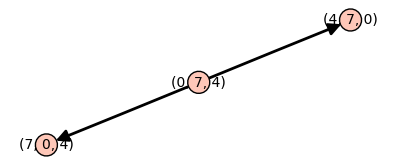
\includegraphics[scale=0.7]{img/p1_1.png}
\end{center}

En el digrafo anterior, est\'{a}n representados los tres estados que hemos listado hasta el momento, el inicial $(0,7,4)$ que tiene como siguientes estados posibles a $(7,0,4)$ y $(4,7,0)$, como v\'{e}rtices y en donde un enlace representa la transici\'{o}n de un estado a otro. \\

Podremos entonces, obtener los siguientes estados de $(7,0,4)$ y $(4,7,0)$. Eso es, en un grafo ilustrado..

\begin {center}
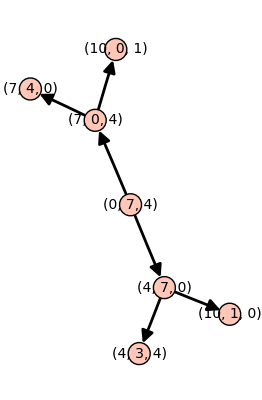
\includegraphics[scale=0.7]{img/p1_2.png}
\end{center}

La pregunta a contestar ser\'{i}a entonces si existe alg\'{u}n v\'{e}rtice i.e. estado que tenga a algun contenedor $a,b$ o $c$ con valor 2. \\ \\

\item �Qu\'{e} algoritmo deber\'{i}a aplicarse para resolver este problema? \\

\textbf{Respuesta:} Deber\'{i}a de aplicarse un algoritmo que genere los siguientes estados posibles, dado un estado inicial, este deber\'{i}a obviar a los estados que ya fueron 
considerados antes. Despu\'{e}s, revisar en cada vertice generado, y los generados de este, si existe una tupla cuyo primer elemento sea 2. \\ \\

\begin{center}
\textit{Algoritmo para generar los proximos estados posibles}
\end{center}

\vspace{0.75cm}
\begin{sageblock}
def getProximosEstados(lista,estadosAnteriores):
    posibles = []
    posible = copy(lista)
    
    if (posible[0]<10):    #si cabe mas en 'a'
        # tratar de pasar de b -> a
        posible[0] += posible[1];
        if (posible[0]>10): #se lleno 'a' antes de vaciar 'c'?
            posible[1] = posible[0] - 10
            posible[0] = 10
        else:             # se vacio b
            posible[1] = 0
            
        #agregarlo si no existe
        if (estadosAnteriores.count(posible)==0):
            posibles.append(posible)
        
        # tratar de pasar de c -> a
        posible = copy(lista)
        posible[0] += posible[2];
        if (posible[0]>10): #se lleno 'a' antes de vaciar 'c'?
            posible[2] = posible[0] - 10
            posible[0] = 10
        else:             # se vacio b
            posible[2] = 0
        
        if (estadosAnteriores.count(posible)==0):
            posibles.append(posible)
    
    posible = copy(lista)
    #si cabe mas en 'b'
    if (posible[1]<7):
        #print 'cabe en b'
        # tratar de pasar de a -> b
        posible[1] += posible[0];
        if (posible[1]>7): #se lleno 'b' antes de vaciar 'a'?
            posible[0] = posible[1] - 7
            posible[1] = 7
        else:             # se vacio a
            posible[0] = 0

        if (estadosAnteriores.count(posible)==0):
            posibles.append(posible)
        
        posible = copy(lista)
        # tratar de pasar de c -> b
        posible[1] += posible[2];
        if (posible[1]>7): #se lleno 'b' antes de vaciar 'a'?
            posible[2] = posible[1] - 7
            posible[1] = 7
        else:             # se vacio a
            posible[2] = 0
        
        if (estadosAnteriores.count(posible)==0):
            posibles.append(posible)
        
    posible = copy(lista)
    #si cabe mas en 'c'
    if (posible[2]<4):
        #print 'cabe en c'
        # tratar de pasar de a -> c
        posible[2] += posible[0];
        if (posible[2]>4): #se lleno 'c' antes de vaciar 'a'?
            posible[0] = posible[2] - 4
            posible[2] = 4
        else:             # se vacio a
            posible[0] = 0
        
        if (estadosAnteriores.count(posible)==0):
            posibles.append(posible)
        
        posible = copy(lista)
        # tratar de pasar de b -> c
        posible[2] += posible[1];
        if (posible[2]>4): #se lleno 'c' antes de vaciar 'b'?
            posible[1] = posible[2] - 4
            posible[2] = 4
        else:             # se vacio a
            posible[2] = 0
    
        if (estadosAnteriores.count(posible)==0):
            posibles.append(posible)
    #print 'devolvio posibles: ', posibles
    return posibles
\end{sageblock}

\vspace{0.75cm}
\begin{center}
\textit{Algoritmo para encontrar la respuesta}
\end{center}
\vspace{0.75cm}
\begin{sageblock}
def existeUnoCon2Litros(lista):
    if (type(lista)==list):
        return lista.count(2)
    else:
        return 0
        
def encontrar(estados,stackTrace):
    encontro = False

    for estado in estados:
        if (not encontro):        
            if (existeUnoCon2Litros(estado)>0):
                global encontro
                encontro = True;
                stackTrace.append(estado)
                print 'encontro, stack trace: ', stackTrace
                return encontro;
                break;
             
            if (not encontro):
                if (type(estado)==list):
                    # si no existe en el stack trace, mandarlo
                    if (stackTrace.count(estado)==0):
                        stackTrace.append(estado)
                        #print 'mando estado i: ',estado
                        encontrar(getProximosEstados(estado,estados),stackTrace)
                else:
                    #print 'mando estado: ',estados
                    stackTrace.append(estados)
                    encontrar(getProximosEstados(estados,[]),stackTrace)
                   
    return encontro

\end{sageblock}

\item Encuentre la respuesta aplicando dicho algoritmo. \\

\textbf{Respuesta:}
\begin{sageblock}
encontro, stack trace:  [[0, 7, 4], [7, 0, 4], [10, 0, 1], [3, 7, 1],
[4, 7, 0], [10, 1, 0], [6, 1, 4], [6, 5, 0], [2, 5, 4]]
True
\end{sageblock} \\ \\

\end{enumerate} 

%Problema 2
\vspace{2cm}
\item [Problema 2] 
Resuelva el problema 107 del Proyecto Euler. \\\\
\textbf{Algoritmo:}\\
\begin{sageblock}
	Grafo = Graph(40)
	matriz = ([[100000000,100000000,100000000,427,668,495,377,678,100000000,177,100000000,100000000,870,100000000,869,624,300,609,131,100000000,251,100000000,100000000,100000000,856,221,514,100000000,591,762,182,56,100000000,884,412,273,636,100000000,100000000,774],[100000000,100000000,262,100000000,100000000,508,472,799,100000000,956,578,363,940,143,100000000,162,122,910,100000000,729,802,941,922,573,531,539,667,607,100000000,920,100000000,100000000,315,649,937,100000000,185,102,636,289],[100000000,262,100000000,100000000,926,100000000,958,158,647,47,621,264,81,100000000,402,813,649,386,252,391,264,637,349,100000000,100000000,100000000,108,100000000,727,225,578,699,100000000,898,294,100000000,575,168,432,833],[427,100000000,100000000,100000000,366,100000000,100000000,635,100000000,32,962,468,893,854,718,427,448,916,258,100000000,760,909,529,311,404,100000000,100000000,588,680,875,100000000,615,100000000,409,758,221,100000000,100000000,76,257],[668,100000000,926,366,100000000,100000000,100000000,250,268,100000000,503,944,100000000,677,100000000,727,793,457,981,191,100000000,100000000,100000000,351,969,925,987,328,282,589,100000000,873,477,100000000,100000000,19,450,100000000,100000000,100000000],[495,508,100000000,100000000,100000000,100000000,100000000,765,711,819,305,302,926,100000000,100000000,582,100000000,861,100000000,683,293,100000000,100000000,66,100000000,27,100000000,100000000,290,100000000,786,100000000,554,817,33,100000000,54,506,386,381],[377,472,958,100000000,100000000,100000000,100000000,100000000,100000000,120,42,100000000,134,219,457,639,538,374,100000000,100000000,100000000,966,100000000,100000000,100000000,100000000,100000000,449,120,797,358,232,550,100000000,305,997,662,744,686,239],[678,799,158,635,250,765,100000000,100000000,100000000,35,100000000,106,385,652,160,100000000,890,812,605,953,100000000,100000000,100000000,79,100000000,712,613,312,452,100000000,978,900,100000000,901,100000000,100000000,225,533,770,722],[100000000,100000000,647,100000000,268,711,100000000,100000000,100000000,283,100000000,172,100000000,663,236,36,403,286,986,100000000,100000000,810,761,574,53,793,100000000,100000000,777,330,936,883,286,100000000,174,100000000,100000000,100000000,828,711],[177,956,47,32,100000000,819,120,35,283,100000000,50,100000000,565,36,767,684,344,489,565,100000000,100000000,103,810,463,733,665,494,644,863,25,385,100000000,342,470,100000000,100000000,100000000,730,582,468],[100000000,578,621,962,503,305,42,100000000,100000000,50,100000000,155,519,100000000,100000000,256,990,801,154,53,474,650,402,100000000,100000000,100000000,966,100000000,100000000,406,989,772,932,7,100000000,823,391,100000000,100000000,933],[100000000,363,264,468,944,302,100000000,106,172,100000000,155,100000000,100000000,100000000,380,438,100000000,41,266,100000000,100000000,104,867,609,100000000,270,861,100000000,100000000,165,100000000,675,250,686,995,366,191,100000000,433,100000000],[870,940,81,893,100000000,926,134,385,100000000,565,519,100000000,100000000,313,851,100000000,100000000,100000000,248,220,100000000,826,359,829,100000000,234,198,145,409,68,359,100000000,814,218,186,100000000,100000000,929,203,100000000],[100000000,143,100000000,854,677,100000000,219,652,663,36,100000000,100000000,313,100000000,132,100000000,433,598,100000000,100000000,168,870,100000000,100000000,100000000,128,437,100000000,383,364,966,227,100000000,100000000,807,993,100000000,100000000,526,17],[869,100000000,402,718,100000000,100000000,457,160,236,767,100000000,380,851,132,100000000,100000000,596,903,613,730,100000000,261,100000000,142,379,885,89,100000000,848,258,112,100000000,900,100000000,100000000,818,639,268,600,100000000],[624,162,813,427,727,582,639,100000000,36,684,256,438,100000000,100000000,100000000,100000000,539,379,664,561,542,100000000,999,585,100000000,100000000,321,398,100000000,100000000,950,68,193,100000000,697,100000000,390,588,848,100000000],[300,122,649,448,793,100000000,538,890,403,344,990,100000000,100000000,433,596,539,100000000,100000000,73,100000000,318,100000000,100000000,500,100000000,968,100000000,291,100000000,100000000,765,196,504,757,100000000,542,100000000,395,227,148],[609,910,386,916,457,861,374,812,286,489,801,41,100000000,598,903,379,100000000,100000000,100000000,946,136,399,100000000,941,707,156,757,258,251,100000000,807,100000000,100000000,100000000,461,501,100000000,100000000,616,100000000],[131,100000000,252,258,981,100000000,100000000,605,986,565,154,266,248,100000000,613,664,73,100000000,100000000,686,100000000,100000000,575,627,817,282,100000000,698,398,222,100000000,649,100000000,100000000,100000000,100000000,100000000,654,100000000,100000000],[100000000,729,391,100000000,191,683,100000000,953,100000000,100000000,53,100000000,220,100000000,730,561,100000000,946,686,100000000,100000000,389,729,553,304,703,455,857,260,100000000,991,182,351,477,867,100000000,100000000,889,217,853],[251,802,264,760,100000000,293,100000000,100000000,100000000,100000000,474,100000000,100000000,168,100000000,542,318,136,100000000,100000000,100000000,100000000,392,100000000,100000000,100000000,267,407,27,651,80,927,100000000,974,977,100000000,100000000,457,117,100000000],[100000000,941,637,909,100000000,100000000,966,100000000,810,103,650,104,826,870,261,100000000,100000000,399,100000000,389,100000000,100000000,100000000,202,100000000,100000000,100000000,100000000,867,140,403,962,785,100000000,511,100000000,1,100000000,707,100000000],[100000000,922,349,529,100000000,100000000,100000000,100000000,761,810,402,867,359,100000000,100000000,999,100000000,100000000,575,729,392,100000000,100000000,388,939,100000000,959,100000000,83,463,361,100000000,100000000,512,931,100000000,224,690,369,100000000],[100000000,573,100000000,311,351,66,100000000,79,574,463,100000000,609,829,100000000,142,585,500,941,627,553,100000000,202,388,100000000,164,829,100000000,620,523,639,936,100000000,100000000,490,100000000,695,100000000,505,109,100000000],[856,531,100000000,404,969,100000000,100000000,100000000,53,733,100000000,100000000,100000000,100000000,379,100000000,100000000,707,817,304,100000000,100000000,939,164,100000000,100000000,616,716,728,100000000,889,349,100000000,963,150,447,100000000,292,586,264],[221,539,100000000,100000000,925,27,100000000,712,793,665,100000000,270,234,128,885,100000000,968,156,282,703,100000000,100000000,100000000,829,100000000,100000000,100000000,822,100000000,100000000,100000000,736,576,100000000,697,946,443,100000000,205,194],[514,667,108,100000000,987,100000000,100000000,613,100000000,494,966,861,198,437,89,321,100000000,757,100000000,455,267,100000000,959,100000000,616,100000000,100000000,100000000,349,156,339,100000000,102,790,359,100000000,439,938,809,260],[100000000,607,100000000,588,328,100000000,449,312,100000000,644,100000000,100000000,145,100000000,100000000,398,291,258,698,857,407,100000000,100000000,620,716,822,100000000,100000000,293,486,943,100000000,779,100000000,6,880,116,775,100000000,947],[591,100000000,727,680,282,290,120,452,777,863,100000000,100000000,409,383,848,100000000,100000000,251,398,260,27,867,83,523,728,100000000,349,293,100000000,212,684,505,341,384,9,992,507,48,100000000,100000000],[762,920,225,875,589,100000000,797,100000000,330,25,406,165,68,364,258,100000000,100000000,100000000,222,100000000,651,140,463,639,100000000,100000000,156,486,212,100000000,100000000,349,723,100000000,100000000,186,100000000,36,240,752],[182,100000000,578,100000000,100000000,786,358,978,936,385,989,100000000,359,966,112,950,765,807,100000000,991,80,403,361,936,889,100000000,339,943,684,100000000,100000000,965,302,676,725,100000000,327,134,100000000,147],[56,100000000,699,615,873,100000000,232,900,883,100000000,772,675,100000000,227,100000000,68,196,100000000,649,182,927,962,100000000,100000000,349,736,100000000,100000000,505,349,965,100000000,474,178,833,100000000,100000000,555,853,100000000],[100000000,315,100000000,100000000,477,554,550,100000000,286,342,932,250,814,100000000,900,193,504,100000000,100000000,351,100000000,785,100000000,100000000,100000000,576,102,779,341,723,302,474,100000000,689,100000000,100000000,100000000,451,100000000,100000000],[884,649,898,409,100000000,817,100000000,901,100000000,470,7,686,218,100000000,100000000,100000000,757,100000000,100000000,477,974,100000000,512,490,963,100000000,790,100000000,384,100000000,676,178,689,100000000,245,596,445,100000000,100000000,343],[412,937,294,758,100000000,33,305,100000000,174,100000000,100000000,995,186,807,100000000,697,100000000,461,100000000,867,977,511,931,100000000,150,697,359,6,9,100000000,725,833,100000000,245,100000000,949,100000000,270,100000000,112],[273,100000000,100000000,221,19,100000000,997,100000000,100000000,100000000,823,366,100000000,993,818,100000000,542,501,100000000,100000000,100000000,100000000,100000000,695,447,946,100000000,880,992,186,100000000,100000000,100000000,596,949,100000000,91,100000000,768,273],[636,185,575,100000000,450,54,662,225,100000000,100000000,391,191,100000000,100000000,639,390,100000000,100000000,100000000,100000000,100000000,1,224,100000000,100000000,443,439,116,507,100000000,327,100000000,100000000,445,100000000,91,100000000,248,100000000,344],[100000000,102,168,100000000,100000000,506,744,533,100000000,730,100000000,100000000,929,100000000,268,588,395,100000000,654,889,457,100000000,690,505,292,100000000,938,775,48,36,134,555,451,100000000,270,100000000,248,100000000,371,680],[100000000,636,432,76,100000000,386,686,770,828,582,100000000,433,203,526,600,848,227,616,100000000,217,117,707,369,109,586,205,809,100000000,100000000,240,100000000,853,100000000,100000000,100000000,768,100000000,371,100000000,540],[774,289,833,257,100000000,381,239,722,711,468,933,100000000,100000000,17,100000000,100000000,148,100000000,100000000,853,100000000,100000000,100000000,100000000,264,194,260,947,100000000,752,147,100000000,100000000,343,112,273,344,680,540,100000000]])
	for i in range(40):
	    for j in range(40):
	        Grafo.add_edge(i,j,matriz[i][j])
			
	peso = lambda e: e[2]
	peso_minimo = sum([a[2] for a in Grafo.min_spanning_tree(weight_function = peso)])
	peso_maximo = sum([sum([b for b in a if b!=100000000]) for a in matriz])/2
	peso_ahorrado = peso_maximo - peso_minimo
	peso_ahorrado
\end{sageblock}

\textit{Respuesta: }259679\\\\

\item [Problema 5] 

Una compa\~{n}\'{i}a tiene sucursales en seis ciudades $C1, C2, \dots , C6$. El costo de transporte de $C_i$ hacia $C_j$ est\'{a} dado por
la entrada $(i, j)$ de la siguiente matriz (donde un costo $\infty$ significa que no hay ruta directa entre esas ciudades):

\[ \left(\begin{array}{rrrrrr}
0 & 50 & \infty & 40 & 25 & 10 \\
50 & 0 & 15 & 20 &  \infty  & 25 \\
 \infty  & 15 & 0 & 10 & 20 &  \infty  \\
40 & 20 & 10 & 0 & 10 & 25 \\
25 &  \infty  & 20 & 10 & 0 & 55 \\
10 & 25 &  \infty  & 25 & 55 & 0
\end{array}\right)\]

La compan\~{n}\'{i}a est\'{a} interesada en preparar una tabla de costos m\'{i}�nimos de transporte entre ciudades. Prepare dicha tabla. \\\\
\textbf{Soluci\'{o}n:}\\

Utilizando el algoritmo de Floyd. 


\begin{sageblock}
def FloydWarshal(M):
    if M.is_square():
        n = len(M.columns())
        for k in range (0,n):
            for i in range (0,n):
                for j in range (0,n):
                    fila = copy(M[i])
                    fila[j] = min(M[i][j] , M[i][k] + M[k][j])
                    M[i] = fila
                    #M[i][j] = min (M[i][j] , 40)
        return M
    else:
        return False
        
        
M5 = matrix([[0,50,10000,40,25,10],[50,0,15,20,10000,25],[10000,15,0,10,20,10000],[40,20,10,0,10,25],[25,10000,20,10,0,55],[10,25,10000,25,55,0]]);

print FloydWarshal(M5)

\end{sageblock}

\textbf{Respuesta:}

\[
\left(\begin{array}{rrrrrr}
0 & 35 & 45 & 35 & 25 & 10 \\
35 & 0 & 15 & 20 & 30 & 25 \\
45 & 15 & 0 & 10 & 20 & 35 \\
35 & 20 & 10 & 0 & 10 & 25 \\
25 & 30 & 20 & 10 & 0 & 35 \\
10 & 25 & 35 & 25 & 35 & 0
\end{array}\right) \]


\end{description}





%\begin{enumerate}[a.] 
%\item {algo}
%\item �Existe alguna secuencia de operaciones que deje exactamente 2 litros en alguno de los contenedores? \\

%\end{enumerate}

\section{}
%\subsection{}



\end{document}  